\documentclass[aspectratio=169]{beamer}

\usetheme{Madrid}
\usecolortheme{default}

\usepackage[utf8]{inputenc}
\usepackage{amsmath,amssymb,amsfonts}
\usepackage{graphicx}
\usepackage{grffile}
\usepackage{booktabs}
\usepackage{tikz}
\usetikzlibrary{arrows.meta,positioning}
\usepackage{url}

% ============================================================
% Paths to experiment outputs (relative to Presentation/)
% ============================================================
\newcommand{\RUNROOT}{../Code/runs_20251213_101931}
\newcommand{\MAINRUN}{dep2030-01-01_2032-01-01_arr2030-05-01_2032-12-26}

% Build a full plot path (ALWAYS single-line when used)
\newcommand{\PLOT}[2]{\RUNROOT/#1/plots/#2}

% ============================================================
% Safe include (macro expansion + detokenize + placeholder)
% ============================================================
\makeatletter
\newcommand{\safeincludegraphics}[2][]{%
	\begingroup
	% Expand macros first (RUNROOT, MAINRUN, etc.)
	\edef\@tmp{#2}%
	% Detokenize so special chars are safe for file tests
	\edef\@figpath{\detokenize\expandafter{\@tmp}}%
	\IfFileExists{\@figpath}{%
		\includegraphics[#1]{\@figpath}%
	}{%
		\fbox{\parbox{0.9\textwidth}{\centering
				\vspace{0.12\textheight}
				\textbf{Missing figure}\\[0.4em]
				\small\texttt{\@figpath}
				\vspace{0.12\textheight}
		}}%
	}%
	\endgroup
}
\makeatother

% ============================================================
% Title info
% ============================================================
\title[Earth--Mars Pork-Chop Surrogates]{Data-Driven Approximation of Earth--Mars Pork-Chop Surfaces}
\author[Scott Nguyen]{Scott Nguyen}
\institute[UNM]{Dept.\ of Electrical \& Computer Engineering \\ University of New Mexico}
\date{ECE 506 Final Project Presentation}

\begin{document}
	
	% ------------------------------------------------------------
	\begin{frame}
		\titlepage
	\end{frame}
	
	% ------------------------------------------------------------
	\begin{frame}{Motivation \& Problem Statement}
		\begin{itemize}
			\item Interplanetary trajectory design requires repeated evaluation of transfer costs over large launch windows.
			\item These trade spaces are visualized using \textbf{pork-chop plots}:
			\[
			\Delta V(\text{departure date},\ \text{time-of-flight})
			\]
			\item Classical workflow:
			\begin{itemize}
				\item Solve Lambert’s problem at every grid point.
				\item Becomes computationally expensive for wide windows or repeated optimization.
			\end{itemize}
			\item \textbf{Project objective}:
			\begin{itemize}
				\item Train a neural-network surrogate to approximate the Earth--Mars pork-chop surface.
				\item Enable fast evaluation, grid search, and optimization using the surrogate.
			\end{itemize}
		\end{itemize}
	\end{frame}
	
	%----------------------------------------------------------
	\begin{frame}{Background \& Related Work}
		\begin{itemize}
			\item \textbf{RL for robust low-thrust trajectories:}
			Zavoli \& Federici formulate Earth--Mars low-thrust transfers as Markov decision processes and train deep RL guidance and control networks that are robust to process noise, navigation uncertainty, and missed-thrust events.
			\item \textbf{Meta-RL for multiple uncertainties:}
			Federici \& Zavoli extend this to meta-reinforcement learning with recurrent networks, learning a closed-loop policy that adapts across environments with mixed dynamic and control uncertainties for a fuel-optimal Earth--Mars transfer.
			\item \textbf{Surrogate NNs for trajectory planning:}
			Ruff et al.\ use neural-network surrogates inside a simulation-based optimization loop to design hypersonic approach-and-landing reference trajectories, showing large reductions in computation time versus direct simulation-based tuning.
			\item This project:
			\begin{itemize}
				\item Adopts the idea of NN surrogates from Ruff et al., but in a simpler supervised setting.
				\item Applies it to an impulsive Earth--Mars Lambert pork-chop rather than low-thrust optimal control.
				\item Focuses on quantifying how well a compact MLP can approximate the $\Delta V$ surface over a 2030--2032 launch window.
			\end{itemize}
		\end{itemize}
	\end{frame}
	
	% ------------------------------------------------------------
	\begin{frame}{Objective Function (What We Minimize)}
		\small
		We solve a two-impulse heliocentric transfer with Lambert's problem (Earth departure, Mars arrival).\\[0.5em]
		
		\textbf{Decision variables:}
		\[
		x \triangleq \begin{bmatrix} t_{\mathrm{dep}} \\ \mathrm{TOF} \end{bmatrix},
		\qquad
		t_{\mathrm{arr}} = t_{\mathrm{dep}} + \mathrm{TOF}
		\]
		
		\textbf{Lambert-based total cost:}
		\[
		J(t_{\mathrm{dep}}, \mathrm{TOF}) \;=\; \Delta V_{\mathrm{tot}}
		\;=\; \left\lVert \mathbf{v}^{\ast}_{\mathrm{dep}} - \mathbf{v}_{E}(t_{\mathrm{dep}})\right\rVert
		\;+\;
		\left\lVert \mathbf{v}_{M}(t_{\mathrm{arr}}) - \mathbf{v}^{\ast}_{\mathrm{arr}}\right\rVert
		\]
		
		where $(\mathbf{v}^{\ast}_{\mathrm{dep}}, \mathbf{v}^{\ast}_{\mathrm{arr}})$ are the Lambert transfer velocities solving
		\[
		(\mathbf{v}^{\ast}_{\mathrm{dep}}, \mathbf{v}^{\ast}_{\mathrm{arr}})
		= \mathrm{Lambert}\!\left(\mathbf{r}_{E}(t_{\mathrm{dep}}),\ \mathbf{r}_{M}(t_{\mathrm{arr}}),\ \mathrm{TOF}\right).
		\]
		
		\textbf{Feasibility / filtering:}\quad solutions with $\Delta V_{\mathrm{tot}} > 20$ km/s are discarded (treated as invalid / NaN).
	\end{frame}
	
	% ------------------------------------------------------------
	\begin{frame}{Workflow Overview}
		\centering
		\resizebox{\textwidth}{!}{%
			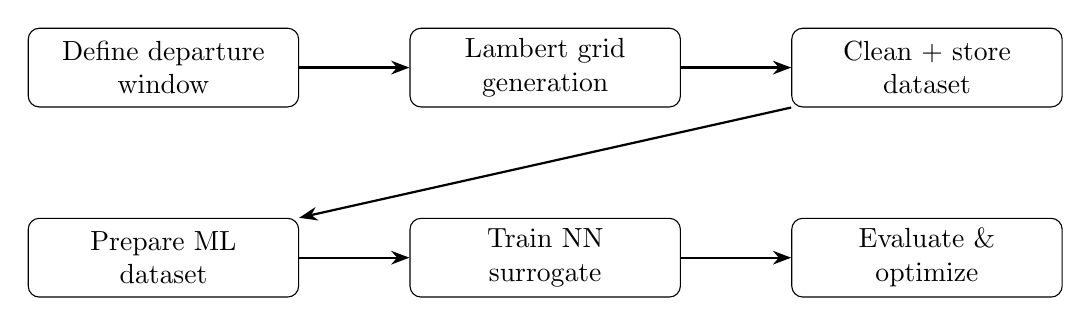
\begin{tikzpicture}[
				block/.style={rectangle, draw, rounded corners, align=center,
					text width=3.2cm, minimum height=1cm},
				arrow/.style={-{Stealth}, thick},
				node distance=1.4cm
				]
				\node[block] (a) {Define departure \\ window};
				\node[block, right=of a] (b) {Lambert grid \\ generation};
				\node[block, right=of b] (c) {Clean + store \\ dataset};
				
				\node[block, below=of a] (d) {Prepare ML \\ dataset};
				\node[block, right=of d] (e) {Train NN \\ surrogate};
				\node[block, right=of e] (f) {Evaluate \& \\ optimize};
				
				\draw[arrow] (a)--(b);
				\draw[arrow] (b)--(c);
				\draw[arrow] (c.south west)--(d.north east);
				\draw[arrow] (d)--(e);
				\draw[arrow] (e)--(f);
		\end{tikzpicture}}
	\end{frame}
	
	% ------------------------------------------------------------
	\begin{frame}{Methods \& How We Compare}
		\small
		\textbf{1) Ground-truth surface (Lambert grid):}
		\begin{itemize}
			\item Sample $t_{\mathrm{dep}}$ daily over a 2-year window ($\sim$731 points).
			\item Sample $\mathrm{TOF}$ over 60 values within the derived feasible arrival bounds.
			\item Evaluate $J(t_{\mathrm{dep}}, \mathrm{TOF})$ at each grid point $\Rightarrow$ pork-chop surface.
		\end{itemize}
		
		\textbf{2) ``True objective'' optimization (continuous):}
		\begin{itemize}
			\item Optimize the same Lambert objective $J(t_{\mathrm{dep}}, \mathrm{TOF})$ over continuous bounds.
			\item Differential Evolution (DE) used to reduce sensitivity to nonconvexity / invalid regions.
			\item Output: best $(t_{\mathrm{dep}}, \mathrm{TOF})$ and optimization history (path over pork-chop).
		\end{itemize}
		
		\textbf{3) Surrogate model (NN regression):}
		\begin{itemize}
			\item Train $\,\widehat{J}(t_{\mathrm{dep}}, \mathrm{TOF})\,$ on valid grid samples only.
			\item Evaluate: MAE/RMSE between $\widehat{J}$ and $J$ on held-out data.
		\end{itemize}
		
		\textbf{4) Surrogate-based optimization (continuous):}
		\begin{itemize}
			\item Minimize $\widehat{J}(t_{\mathrm{dep}}, \mathrm{TOF})$ with DE.
			\item \textbf{Key comparison:} report both (i) predicted optimum $\widehat{J}$ and (ii) \textbf{true} $J$ evaluated at that surrogate optimum.
		\end{itemize}
	\end{frame}
	
	% ------------------------------------------------------------
	\begin{frame}{Dataset Generation}
		\begin{itemize}
			\item Earth--Mars Lambert transfers using \texttt{poliastro}.
			\item Departure dates sampled daily over 2-year windows.
			\item Time-of-flight sampled uniformly within feasible arrival bounds (derived from arrival window).
			\item Invalid solutions ($\Delta V > 20$ km/s) removed.
			\item Multiple windows evaluated:
			\[
			2030\text{--}2032,\ 2032\text{--}2034,\ 2034\text{--}2036,\ 2036\text{--}2038,\ 2038\text{--}2040
			\]
		\end{itemize}
	\end{frame}
	
	% ------------------------------------------------------------
	\begin{frame}{Run Summary (All Windows)}
		\small
		\centering
		\begin{tabular}{lcccc}
			\toprule
			\textbf{Window} & \textbf{Grid min} & \textbf{True opt min} & \textbf{Surrogate MAE} & \textbf{Surrogate RMSE} \\
			\midrule
			2030--2032 & 6.7009 & 6.6445 & 0.7313 & 1.2269 \\
			2032--2034 & 6.1420 & 6.1211 & 0.7985 & 1.3743 \\
			2034--2036 & 5.5770 & 5.5707 & 1.5362 & 3.0171 \\
			2036--2038 & 6.6032 & 6.6002 & 1.5831 & 3.1374 \\
			2038--2040 & 5.7429 & 5.7125 & 1.4953 & 2.5518 \\
			\bottomrule
		\end{tabular}
	\end{frame}
	
	% ------------------------------------------------------------
	\begin{frame}{Baseline Pork-Chop Surface (Lambert)}
		\centering
		\safeincludegraphics[width=0.92\textwidth]{\PLOT{\MAINRUN}{porkchop_2030-01-01_2032-01-01.png}}
	\end{frame}
	
	\begin{frame}{True Objective Optimization}
		\centering
		\safeincludegraphics[width=0.92\textwidth]{\PLOT{\MAINRUN}{porkchop_2030-01-01_2032-01-01_optpath.png}}
	\end{frame}
	
	\begin{frame}{Surrogate Model Evaluation}
		\centering
		\safeincludegraphics[width=\textwidth]{\PLOT{\MAINRUN}{porkchop_triptych_dep20300101-20320101_arr20300501-20321226.png}}
	\end{frame}
	
	\begin{frame}{Error Distribution}
		\centering
		\safeincludegraphics[width=0.75\textwidth]{\PLOT{\MAINRUN}{porkchop_error_histogram_dep20300101-20320101_arr20300501-20321226.png}}
	\end{frame}
	
	\begin{frame}{Four-Minima Comparison}
		\centering
		\safeincludegraphics[width=0.92\textwidth]{\PLOT{\MAINRUN}{porkchop_four_mins_dep20300101-20320101_arr20300501-20321226.png}}
	\end{frame}
	
	% ============================================================
	% BACKUP
	% ============================================================
	\appendix
	\section{Backup}
	
	% 2032--2034
	\begin{frame}{Backup: 2032--2034 Lambert Pork-Chop}
		\centering
		\safeincludegraphics[width=0.92\textwidth]{\PLOT{dep2032-01-01_2034-01-01_arr2032-05-01_2034-12-26}{porkchop_2032-01-01_2034-01-01.png}}
	\end{frame}
	
	\begin{frame}{Backup: 2032--2034 True Objective Optimization}
		\centering
		\safeincludegraphics[width=0.92\textwidth]{\PLOT{dep2032-01-01_2034-01-01_arr2032-05-01_2034-12-26}{porkchop_2032-01-01_2034-01-01_optpath.png}}
	\end{frame}
	
	\begin{frame}{Backup: 2032--2034 Surrogate Triptych}
		\centering
		\safeincludegraphics[width=\textwidth]{\PLOT{dep2032-01-01_2034-01-01_arr2032-05-01_2034-12-26}{porkchop_triptych_dep20320101-20340101_arr20320430-20341227.png}}
	\end{frame}
	
	\begin{frame}{Backup: 2032--2034 Error Histogram}
		\centering
		\safeincludegraphics[width=0.75\textwidth]{\PLOT{dep2032-01-01_2034-01-01_arr2032-05-01_2034-12-26}{porkchop_error_histogram_dep20320101-20340101_arr20320430-20341227.png}}
	\end{frame}
	
	\begin{frame}{Backup: 2032--2034 Four-Minima Comparison}
		\centering
		\safeincludegraphics[width=0.92\textwidth]{\PLOT{dep2032-01-01_2034-01-01_arr2032-05-01_2034-12-26}{porkchop_four_mins_dep20320101-20340101_arr20320430-20341227.png}}
	\end{frame}
	
	% ============================================================
	% 2034--2036
	% ============================================================
	\begin{frame}{Backup: 2034--2036 Lambert Pork-Chop}
		\centering
		\safeincludegraphics[width=0.92\textwidth]{\PLOT{dep2034-01-01_2036-01-01_arr2034-05-01_2036-12-26}{porkchop_2034-01-01_2036-01-01.png}}
	\end{frame}
	
	\begin{frame}{Backup: 2034--2036 True Objective Optimization}
		\centering
		\safeincludegraphics[width=0.92\textwidth]{\PLOT{dep2034-01-01_2036-01-01_arr2034-05-01_2036-12-26}{porkchop_2034-01-01_2036-01-01_optpath.png}}
	\end{frame}
	
	\begin{frame}{Backup: 2034--2036 Surrogate Triptych}
		\centering
		\safeincludegraphics[width=\textwidth]{\PLOT{dep2034-01-01_2036-01-01_arr2034-05-01_2036-12-26}{porkchop_triptych_dep20340101-20360101_arr20340501-20361226.png}}
	\end{frame}
	
	\begin{frame}{Backup: 2034--2036 Error Histogram}
		\centering
		\safeincludegraphics[width=0.75\textwidth]{\PLOT{dep2034-01-01_2036-01-01_arr2034-05-01_2036-12-26}{porkchop_error_histogram_dep20340101-20360101_arr20340501-20361226.png}}
	\end{frame}
	
	\begin{frame}{Backup: 2034--2036 Four-Minima Comparison}
		\centering
		\safeincludegraphics[width=0.92\textwidth]{\PLOT{dep2034-01-01_2036-01-01_arr2034-05-01_2036-12-26}{porkchop_four_mins_dep20340101-20360101_arr20340501-20361226.png}}
	\end{frame}
	
	% ============================================================
	% 2036--2038
	% ============================================================
	\begin{frame}{Backup: 2036--2038 Lambert Pork-Chop}
		\centering
		\safeincludegraphics[width=0.92\textwidth]{\PLOT{dep2036-01-01_2038-01-01_arr2036-05-01_2038-12-26}{porkchop_2036-01-01_2038-01-01.png}}
	\end{frame}
	
	\begin{frame}{Backup: 2036--2038 True Objective Optimization}
		\centering
		\safeincludegraphics[width=0.92\textwidth]{\PLOT{dep2036-01-01_2038-01-01_arr2036-05-01_2038-12-26}{porkchop_2036-01-01_2038-01-01_optpath.png}}
	\end{frame}
	
	\begin{frame}{Backup: 2036--2038 Surrogate Triptych}
		\centering
		\safeincludegraphics[width=\textwidth]{\PLOT{dep2036-01-01_2038-01-01_arr2036-05-01_2038-12-26}{porkchop_triptych_dep20360101-20380101_arr20360430-20381227.png}}
	\end{frame}
	
	\begin{frame}{Backup: 2036--2038 Error Histogram}
		\centering
		\safeincludegraphics[width=0.75\textwidth]{\PLOT{dep2036-01-01_2038-01-01_arr2036-05-01_2038-12-26}{porkchop_error_histogram_dep20360101-20380101_arr20360430-20381227.png}}
	\end{frame}
	
	\begin{frame}{Backup: 2036--2038 Four-Minima Comparison}
		\centering
		\safeincludegraphics[width=0.92\textwidth]{\PLOT{dep2036-01-01_2038-01-01_arr2036-05-01_2038-12-26}{porkchop_four_mins_dep20360101-20380101_arr20360430-20381227.png}}
	\end{frame}
	
	% ============================================================
	% 2038--2040
	% ============================================================
	\begin{frame}{Backup: 2038--2040 Lambert Pork-Chop}
		\centering
		\safeincludegraphics[width=0.92\textwidth]{\PLOT{dep2038-01-01_2040-01-01_arr2038-05-01_2040-12-26}{porkchop_2038-01-01_2040-01-01.png}}
	\end{frame}
	
	\begin{frame}{Backup: 2038--2040 True Objective Optimization}
		\centering
		\safeincludegraphics[width=0.92\textwidth]{\PLOT{dep2038-01-01_2040-01-01_arr2038-05-01_2040-12-26}{porkchop_2038-01-01_2040-01-01_optpath.png}}
	\end{frame}
	
	\begin{frame}{Backup: 2038--2040 Surrogate Triptych}
		\centering
		\safeincludegraphics[width=\textwidth]{\PLOT{dep2038-01-01_2040-01-01_arr2038-05-01_2040-12-26}{porkchop_triptych_dep20380101-20400101_arr20380501-20401226.png}}
	\end{frame}
	
	\begin{frame}{Backup: 2038--2040 Error Histogram}
		\centering
		\safeincludegraphics[width=0.75\textwidth]{\PLOT{dep2038-01-01_2040-01-01_arr2038-05-01_2040-12-26}{porkchop_error_histogram_dep20380101-20400101_arr20380501-20401226.png}}
	\end{frame}
	
	\begin{frame}{Backup: 2038--2040 Four-Minima Comparison}
		\centering
		\safeincludegraphics[width=0.92\textwidth]{\PLOT{dep2038-01-01_2040-01-01_arr2038-05-01_2040-12-26}{porkchop_four_mins_dep20380101-20400101_arr20380501-20401226.png}}
	\end{frame}
	
	%----------------------------------------------------------
	\begin{frame}{References}
		\tiny
		\begin{thebibliography}{00}
			\bibitem{zavoli2021}
			A.~Zavoli and L.~Federici,
			``Reinforcement Learning for Low-Thrust Trajectory Design of Interplanetary Missions,''
			AAS~20-616, preprint, 2020.
			
			\bibitem{ruff2023}
			E.~Ruff, R.~Russell, M.~Stoeckle, P.~Miotto, and J.~P.~How,
			``Surrogate Neural Networks for Efficient Simulation-based Trajectory Planning Optimization,''
			arXiv preprint arXiv:2303.17468, 2023.
			
			\bibitem{federici2024}
			L.~Federici and A.~Zavoli,
			``Robust Interplanetary Trajectory Design under Multiple Uncertainties via Meta-Reinforcement Learning,''
			\emph{Acta Astronautica}, 2024.
		\end{thebibliography}
	\end{frame}
	
	%----------------------------------------------------------
	\begin{frame}
		\centering
		\Huge Questions?
	\end{frame}
	
\end{document}
